\section{Turbulent Flows}

In the realm of engineering, there is often a need to predict the behavior of fluid flow in and around engineered products.
These situations can range from simulating the flow around an airplane, to simulating the flow through the cooling system in a laptop.
Computational Fluid Dynamics (CFD) is the field of study that involves the use of computers and complex numerical analysis techniques to solve the non-linear Navier-Stokes equations on the flow domain of interest.
As computational capabilities have increased over the past few decades, so has the reliance on the predictive capability of CFD simulations. 

This is made more difficult due to turbulence.
The range of length, and time scales that need to be resolved through spatial, and temporal discretization make it computationally intractable to solve exactly, i.e. without any simplifying models.
Most flows of engineering interest are plagued by turbulence.
The difficulty in solving these flows exactly has paved the way for the development of a hierarchy of solution techniques that trade computational cost for prediction accuracy. 

\begin{figure}
    \center
    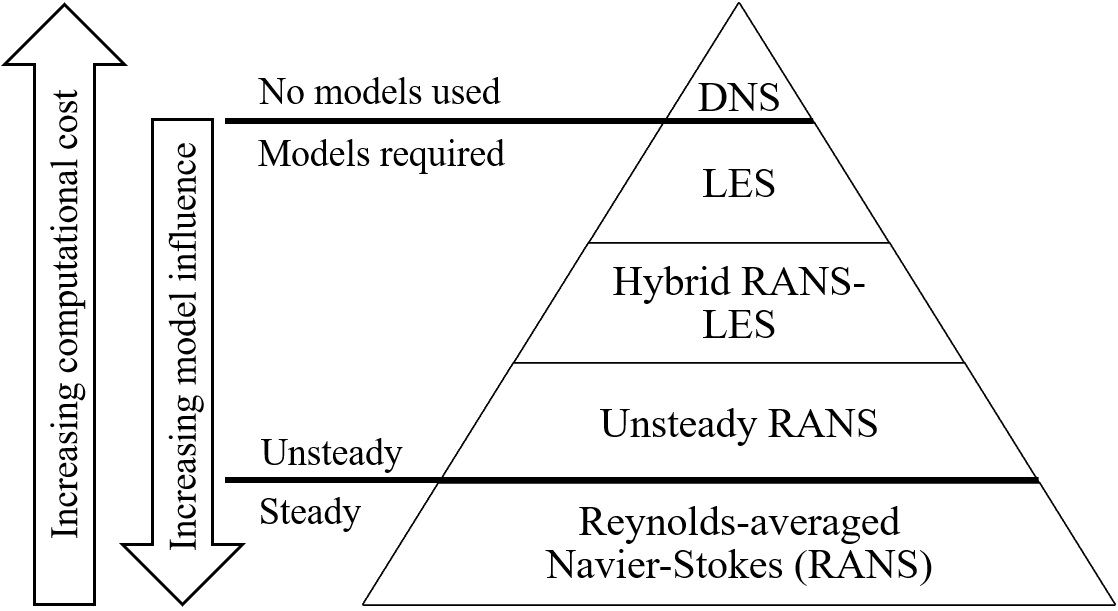
\includegraphics[width=0.75\textwidth]{suthesis/images/solution_heirarchy_simple.png}
    \caption{Hierarchy of CFD solution techniques in order of increasing computational cost and decreasing model influence. \label{fig:cfd_types}}
\end{figure}

Figure \ref{fig:cfd_types} presents this hierarchy in the form of a pyramid.
Sitting at the top of this pyramid are Direct Numerical Simulations, or DNS.
These calculations do not employ any mathematical models and resolve all spatial and temporal time scales to give an exact reproduction of the fluid behavior.
These time-varying (unsteady) simulations are computationally expensive and memory intensive.
At the time of writing, DNS calculations are only possible at low Reynolds numbers and for simple geometries such as flat plates \cite{hoyas_reynolds_2008}, and channels \cite{laval_marquillie_dns_channel,marquillie_instability_2011}.
This disqualifies the use of DNS, in its current state, for practical engineering applications. 

Below DNS, in Figure \ref{fig:cfd_types}, lie Large Eddy Simulations (LES) and Hybrid RANS-LES simulations.
These unsteady simulations resolve some, but not all, of the scales of turbulence.
Any time and length scales that aren't resolved, are modeled using some simplifying assumptions \cite{pope_2000}.
These solution methodologies allow for the fine-tuning of the desired influence of simplifying models through the chosen level of spatial and temporal discretization.
They are in the process of being adopted by industry for specific use cases such as performance predictions for high-lift configuration aircraft \cite{rumsey2019overview}, or engine simulations. 

At the base of the pyramid is the most widely used method in industry, Reynolds-averaged Navier-Stokes (RANS) simulation.
These simulations suffer the most from modeling inaccuracies.
They assume that the flow is steady (no time-dependent variation in flow), and require simplifying turbulence models that aggregate the effects of the turbulent eddies that would be present in the flow.
This significantly reduces the computational cost but inhibits the flow features that can be captured by the simulations.
While its unsteady counterpart can resolve some of the time variation of the flow, turbulence modeling is still required which affects the prediction accuracy.
Steady RANS simulations are very computationally efficient and can be used for expensive undertakings such as iterative aerodynamic shape optimization \cite{lyu2015aerodynamic}, and aircraft database generation \cite{wendorff_combining_2016}.
This chapter will focus on quantifying the uncertainties that are injected by turbulence models that are employed in RANS simulations. 